\documentclass[aspectratio=169]{beamer}
\usepackage{ITMOtheme}
\usepackage[utf8]{inputenc}
\usepackage[english,russian]{babel}
\usepackage{wrapfig}

% Подключите этот пакет, чтобы использовать русский язык.
%\usepackage[english,russian]{babel}

% Если будет предупреждение "Package hyperref Warning: Glyph not defined in PD1 encoding"
%\hypersetup{unicode=true}


%Use this package to automatically format references.
% \usepackage[style=mla]{biblatex}
% \addbibresource{references.bib}

\graphicspath{{./media/}}

%\titlegraphic{\includegraphics[scale=.8]{itmo_logo_rus_vert_blue.pdf}}

% use \title[short title]{full title}
\title[Выпускная квалификационная работа]{Разработка программы
автоматизированного построения полётного задания для управления группой БПЛА}

%\subtitle[short subtitle]{long subtitle}

\author{Де ла Пенья Смирнов Ярослав, г. К3400}
%\supervisor[Овчинников Г.Р.]{Овчинников Георгий Ревмирович}
\newcommand{\supervisor}{Овчинников Георгий Ревмирович, к.т.н.}

%\institute[short institute]{long institute}

\where{Санкт-Петербург}
\date{2020}

%I don’t know if this affects anything.
\subject{example}
\keywords{ITMO University, UAV}


\begin{document}

% \begin{frame}[plain]
%     \titlepage
% \end{frame}


% You can use custom title, if you want.
\begin{frame}[plain]
	\itmopolygons{
	\vfill
		\includegraphics[height=0.2\paperheight]{itmo_logo_rus_vert_blue}
	\vfill
		\usebeamerfont{title}{  \inserttitle\par}
	\vfill
		\usebeamerfont{subtitle}{\insertsubtitle\par}
	\vfill
    Автор: {\insertauthor} \\
    Руководитель: {\supervisor} \par
	\vfill
		\insertinstitute\par
	\vfill
		\insertplace  \;  \insertdate
}
\end{frame}


\begin{frame}{Цель}
  Разработать прототип программного обеспечения для автоматизированного
  построения полётного задания группы БПЛА.
\end{frame}


\begin{frame}{Задачи}
  \begin{itemize}
    \item исследовать и изучить предметную область и теоретические основы темы;
    \item определить общие требования к ПО;
    \item выбрать и изучить оптимальные компоненты и библиотеки для реализации ПО;
    \item выбрать оптимальный язык программирования для реализации ПО;
    \item спроектировать и разработать архитектуру для взаимодействия разных
      компонентов;
    \item разработать прототип ПО для построения полётного задания для управления
      группой БПЛА.
  \end{itemize}
\end{frame}


\begin{frame}{Актуальность темы}
  \begin{itemize}
    \item рост спроса на БПЛА;
    \item появление новых задач;
    \item требования к повышенной автономности БПЛА;
    \item развитие технологий;
  \end{itemize}
\end{frame}


\begin{frame}{Обзор предметной области}
  \begin{figure}[!h]
    \begin{center}
      \includegraphics[height=0.7\textheight]{diag-elems}
    \end{center}
  \end{figure}
\end{frame}


\begin{frame}{Обзор предметной области}
  \begin{wrapfigure}{r}{0.5\textwidth}
    \begin{center}
      \includegraphics[width=0.4\textwidth]{uav-inspect}
    \end{center}
  \end{wrapfigure}
  Выполняемые задания:

  \begin{itemize}
    \item дистанционное зондирование
    \item промышленное обследование
    \item воздушная фотография и видеосъёмка
    \item разведка
    \item метеорология
    \item доставка грузов
  \end{itemize}
\end{frame}


\begin{frame}{Обзор архитектуры системы управления БПЛА}
  \begin{center}
    \includegraphics[height=0.7\textheight]{diag-uav-hw}
  \end{center}
\end{frame}


\begin{frame}{Обзор архитектуры системы управления БПЛА}
  \begin{center}
    \includegraphics[height=0.7\textheight]{diag-uav-sil}
  \end{center}
\end{frame}


\begin{frame}{Требования к ПО}
  \begin{itemize}
    \item совместимость с Linux/Unix
    \item язык программирования с развитой экосистемой
    \item компоненты с свободной лицензией
    \item протоколы коммуникаций использующие существующие сетевые стеки
  \end{itemize}
\end{frame}


\begin{frame}{Компоненты для реализации ПО}
  \begin{itemize}
    \item язык программирования JavaScript
    \item ОС Ubuntu Linux 18.04
    \item автопилот PX4
    \item протокол MAVLink
    \item библиотека React
    \item библиотека Redux
    \item фреймворк Electron
    \item платформа Cesium
  \end{itemize}
\end{frame}


\begin{frame}{Архитектура системы}
  \begin{figure}[!h]
    \begin{center}
      \includegraphics[height=0.7\textheight]{diag-arch-sys}
    \end{center}
  \end{figure}
\end{frame}


\begin{frame}{Архитектура ПО}
  \begin{figure}[!h]
    \begin{center}
      \includegraphics[height=0.7\textheight]{diag-arch-prog}
    \end{center}
  \end{figure}
\end{frame}


\begin{frame}{Разработка ПО}
  Файловая структура:

  \begin{itemize}
    \item \texttt{actions/}
    \item \texttt{components/}
    \item \texttt{mavlink/}
    \item \texttt{reducers/}
    \item \texttt{app.js}
    \item \texttt{index.js}
    \item \texttt{main.js}
  \end{itemize}
\end{frame}


\begin{frame}{Разработка ПО}
  Действия и функции-редукторы:

  \begin{itemize}
    \item \texttt{uav-connect.js}
    \item \texttt{uav-disconnect.js}
    \item \texttt{waypoint-add.js}
    \item \texttt{waypoint-del.js}
    \item \texttt{waypoint-edit.js}
    \item \texttt{uav-location-update.js}
    \item \texttt{mavlink-message-rcv.js}
    \item \texttt{mavlink-message-send.js}
  \end{itemize}
\end{frame}


\begin{frame}{Разработка ПО}
  \begin{wrapfigure}{r}{0.5\textwidth}
    \begin{center}
      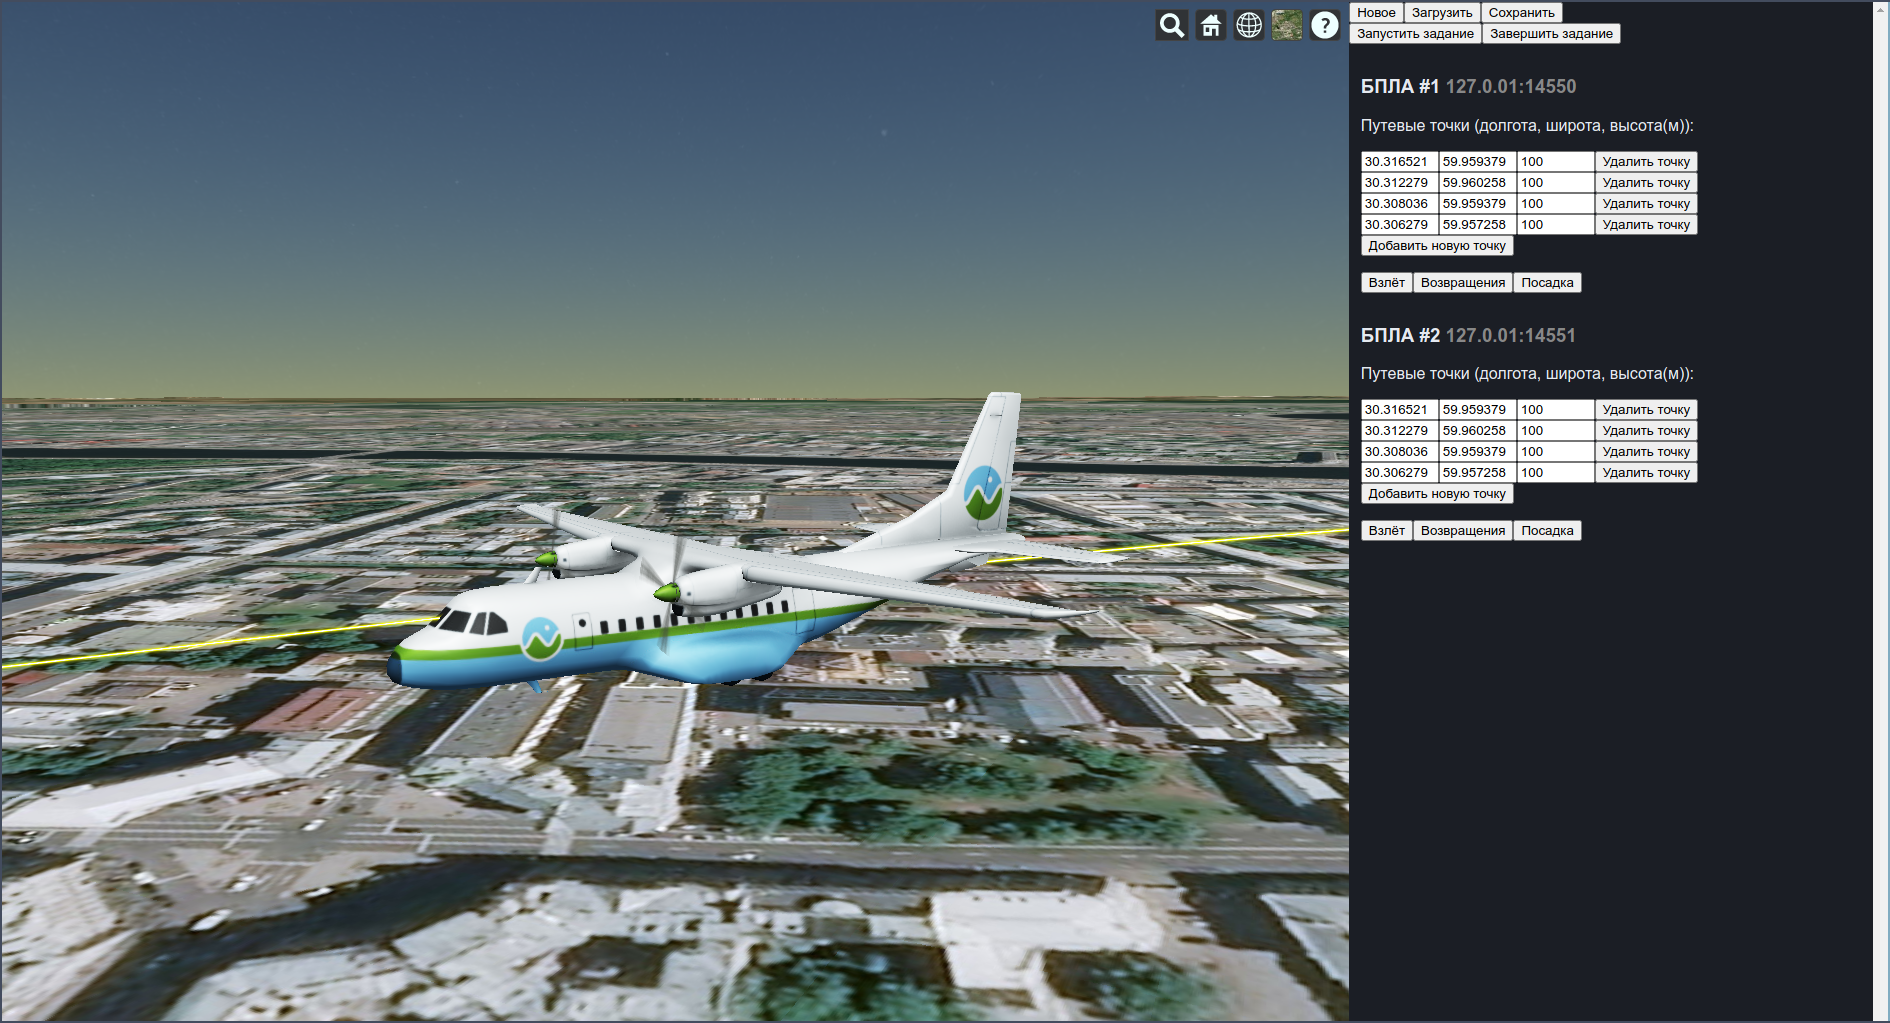
\includegraphics[width=0.4\textwidth]{gui}
    \end{center}
  \end{wrapfigure}
  Компоненты ГПИ:

  \begin{itemize}
    \item \texttt{<CesiumViewer />}
    \item \texttt{<Panel />}
      \begin{itemize}
        \item \texttt{<Aircraft />}
        \item \texttt{<Waypoint />}
      \end{itemize}
  \end{itemize}
\end{frame}


\begin{frame}{Заключение}
  \begin{itemize}
    \item определены основные применения и направления систем беспилотных
      летательных аппаратов;
    \item были анализированы перспективы развития систем БПЛА;
    \item определены основные элементы систем БПЛА;
    \item выбраны необходимые элементы для разработки ПО;
    \item спроектирована архитектура системы и ПО;
    \item разработан прототип программы автоматизированного построения полётного
      задания для управления группой БПЛА.
  \end{itemize}
\end{frame}


\begin{frame}[plain]
    \itmopolygons{
        \vfill
        \Huge{Спасибо за внимание}
        \vfill
        \includegraphics[scale=.5]{slogan.pdf}
    }
\end{frame}

% Use this command to manually change number of pages.
%\setcounter{page}{11}

\end{document}
